\documentclass{ximera}


\author{Anna Davis} \title{MTH 240 Test 2} 

\begin{document}

\begin{abstract}

\end{abstract}
\maketitle
 \textit{You have 1 hour and 50 minutes to complete this test.  Each answer is worth 1 point.}
\begin{problem}\label{prob:mth240exam2prob4}
Complete the following statements.
\begin{enumerate}
\item
If $f'(x)<0$ on the interval $(a, b)$, then $f$ is $\answer{decreasing}$ on $(a, b)$.
\item
If $f'(x)>0$ on the interval $(a, b)$, then $f$ is $\answer{increasing}$ on $(a, b)$.
\end{enumerate}
\end{problem}

\begin{problem}\label{prob:mth240exam2prob1}
Let $$f(x)=x^3-3x^2-72x-1$$
Find the first derivative:
$$f'(x)=\answer{3x^2-6x-72}$$
First order critical numbers are (in increasing order):
$$x=\answer{-4}\quad x=\answer{6}$$
The corresponding critical points are:
$$(\answer{-4}, \answer{175}),\quad (\answer{6}, \answer{-325})$$
The function is increasing on the intervals:
$$(\answer{-\infty},\answer{-4}), (\answer{6}, \answer{\infty})$$
The function is decreasing on the interval:
$$(\answer{-4},\answer{6})$$
Find the second derivative:
$$f''(x)=\answer{6x-6}$$
Second order critical number is:
$$x=\answer{1}$$
Second order critical point is:
$$(\answer{1}, \answer{-75})$$
The graph is concave up on the interval
$$(\answer{1}, \answer{\infty})$$
The graph is concave down on the interval
$$(\answer{-\infty}, \answer{1})$$
\end{problem}

\begin{problem}\label{prob:mth240exam2prob2}
An island is located 1000 feet away from a coastal highway.  A car traveling at 88 ft/sec is approaching point $A$, as shown in the diagram.  How fast is the distance between the car and the island changing when the car is 800 feet away from point $A$?
\begin{image}
   
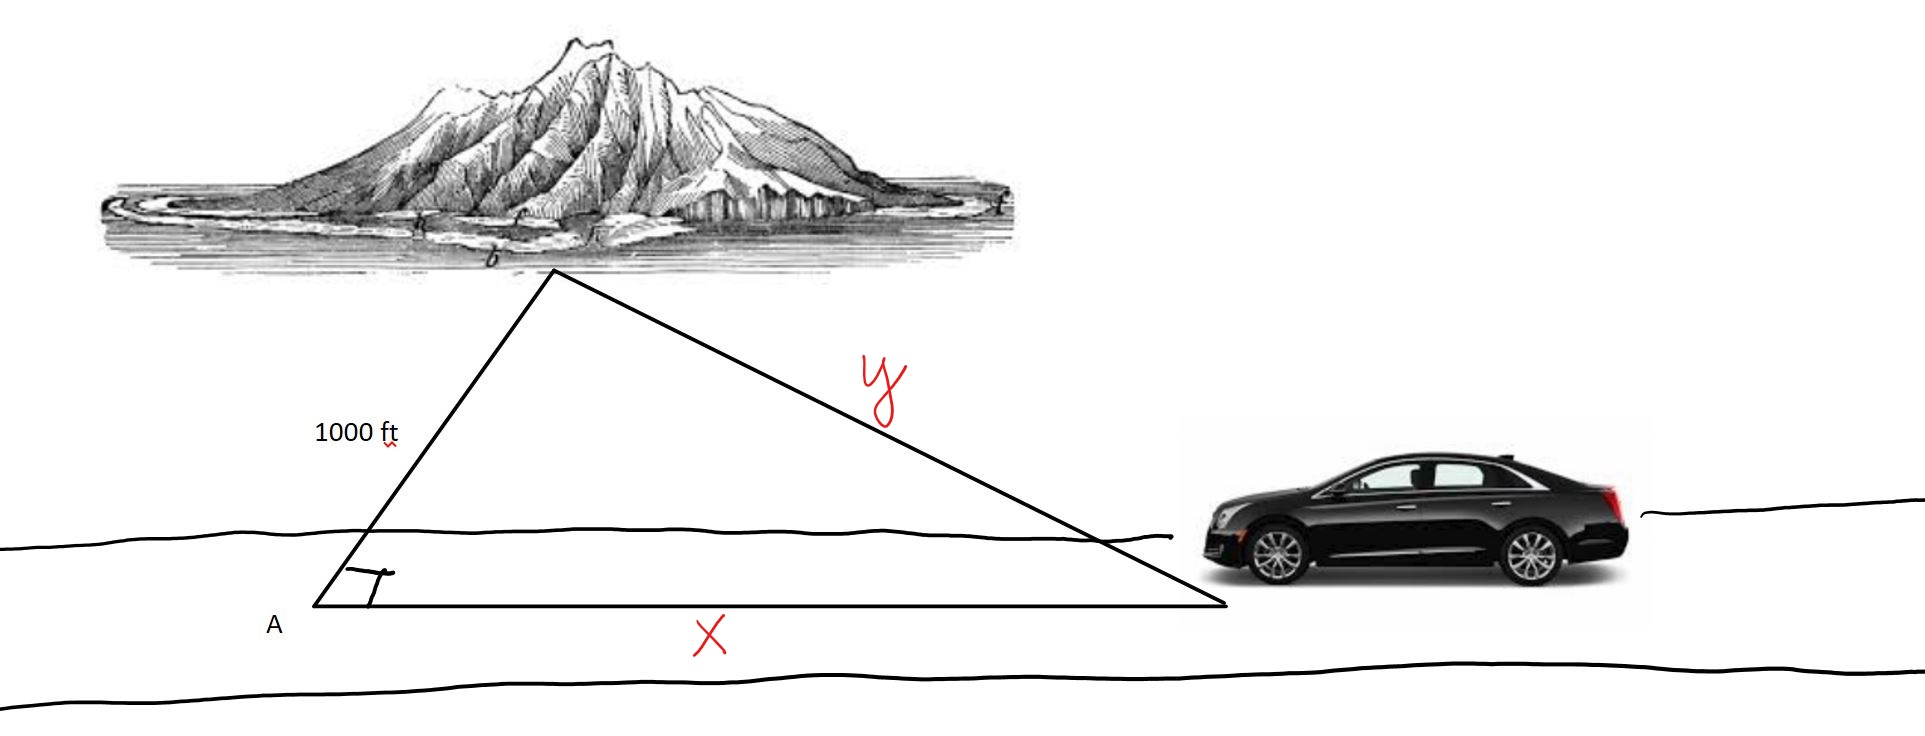
\includegraphics[height=1in]{Inkedtest2image4.jpg}~
 
\end{image}

Given rate: $\answer{\frac{dx}{dt}}=\answer{-88}$.

Find rate:  $\answer{\frac{dy}{dt}}$

Relationship between $\answer{x}$ and $\answer{y}$:

$$\answer{x^2}+1000^2=\answer{y^2}$$

When $x=800$, $y=\answer[tolerance=1]{1280.62}$.

The distance between the car and the island is changing at the rate of $\answer[tolerance=1]{-55}$ feet per second.
\end{problem}

\begin{problem}\label{prob:mth240exam2prob3}
A rectangular trough is to be constructed from a 200 ft by 12 ft sheet of metal by folding up the sides, as shown.  Use calculus to find the largest possible volume of flowing water that the trough can contain.

\begin{image}
   
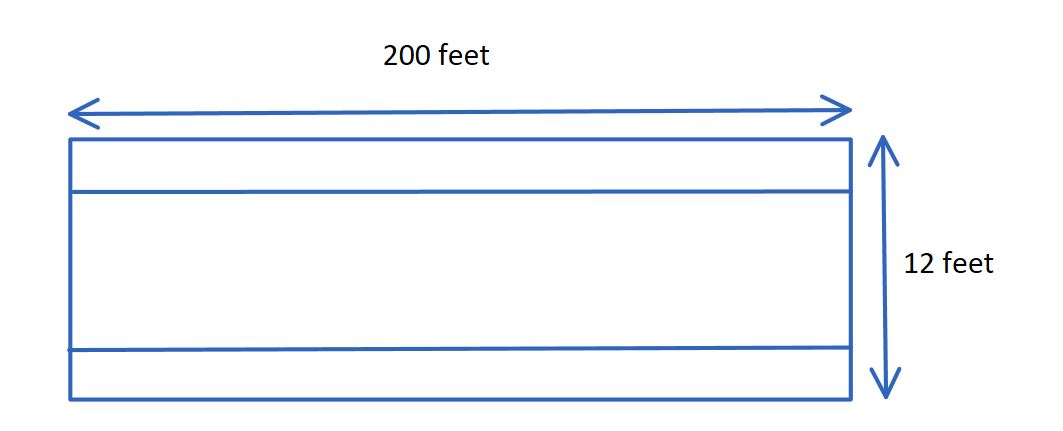
\includegraphics[height=1in]{test2image2.jpg}~
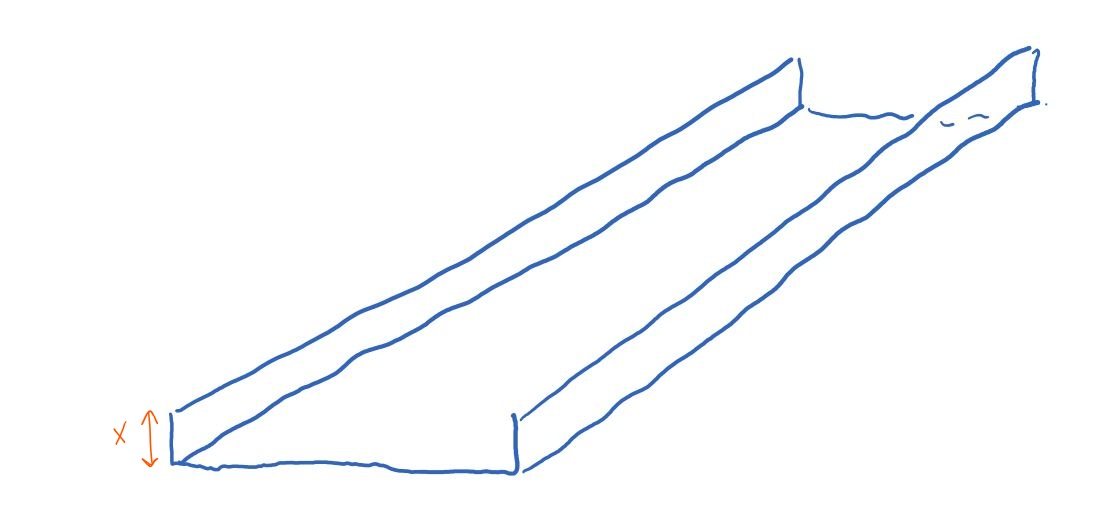
\includegraphics[height=1in]{Inkedtest2image3.jpg}~
 
\end{image}
Volume of the trough:
$$V(x)=\answer{200x(12-2x)}$$
Find the derivative:
$$V'(x)=\answer{-800x+2400}$$
Value of $x$ that gives the largest volume:
$$x=\answer{3}$$
Largest possible volume:
$$V=\answer{3600}\mbox{ square feet}$$

\end{problem}

\begin{problem}\label{prob:mth240exam2prob5}
The radius of a circle was measured to be 12 cm with a possible error in measurement of at most $\pm 0.1$ cm.  Use differentials to estimate the maximum possible error in the computed area of the circle.

Estimated maximum error in computed area is $\pm\answer[tolerance=0.5]{2.4\pi}$ $cm^2$.
\end{problem}

\begin{problem}\label{prob:mth240exam2prob6}
Find the first and second derivatives of $f(x)=x^2e^x$
$$f'(x)=\answer{2xe^x+x^2e^x}$$
$$f''(x)=\answer{2e^x+4xe^x+x^2e^x}$$
\end{problem}

\begin{problem}\label{prob:mth240exam2prob7}
Use linearization to estimate $\sqrt{10}$.

The function I will use is:
$$f(x)=\answer{\sqrt{x}}$$

The derivative of the function is:
$$f'(x)=\answer{0.5x^{-0.5}}$$

Next, I need to find the tangent line to the graph of $f$ at $x=\answer{9}$.

The slope of the tangent line is (enter exact fraction; no decimals) $\answer{\frac{1}{6}}$.

The equation of the tangent line is:
$$y=\answer{\frac{1}{6}x+\frac{3}{2}}$$
Enter exact fraction for the final answer:
$$\sqrt{10}\approx \answer{\frac{19}{6}}$$
\end{problem}

\begin{problem}\label{prob:mth240exam2prob8}
The graph of $f(x)=0.25x^3-x+1$ is shown in the figure.  Find the absolute maximum and the absolute minimum value of the function on the interval $[-2, 1]$.
 
\[
\graph[xmin=-5,xmax=5,ymin=-5,ymax=5]{f(x)=0.25x^3-x+1} 
\]

    Absolute max is $\answer[tolerance=0.01]{1.77}$ at $x=\answer[tolerance=0.01]{-1.155}$.
    
    Absolute min is $\answer{0.25}$ at $x=\answer{1}$.
\end{problem}

\begin{problem}\label{prob:mth240exam2prob9}
Find the equation of the tangent line to the curve given below at $(1,1)$.
$$xy+x^2y^2=2x$$

Start by finding $\frac{dy}{dx}$.
$$\frac{dy}{dx}=\answer{\frac{2-y-2xy^2}{x+2x^2y}}$$
Slope of the tangent line at $(1,1)$ is:
$$m=\answer{\frac{-1}{3}}$$
Equation of the tangent line is:
$$y=-\frac{1}{3}x+\frac{4}{3}$$
\end{problem}
\end{document} 